\section{Qualitative Insights on Leaderboards}
\label{ch:isicle:interp}

\name{} also helps qualitative analysis of \itms{} and \subjs{}.
First, \irt{} identifies overfitting and generalizes partitioning datasets by \diff{}.
Then we show that---like in educational testing---\irt{} identifies good and bad \itms{}.

\subsection{Guiding Analysis with IRT}

\begin{figure*}[t]
    \centering
    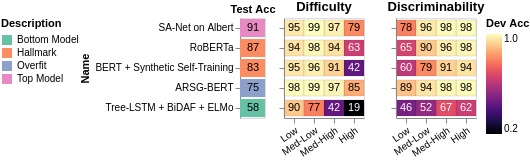
\includegraphics[width=.8\textwidth]{irt_confusion}
    \caption{
        We partition evaluation data by \irt{} \diff{} and
        \discability{} with accuracy in each quartile.
        Most improvements in high-accuracy systems come from getting
        high-difficulty questions right.
        \Itms{} with low \discability{} (and thus prone to annotation errors) are difficult for all \subjs{} except the overfit \abr{args-bert} model.
        We include top-performing \squad{} \subjs{}, several notable
        \subjs{} (systems), and a pair from the bottom of the leaderboard.
    }
    \label{fig:confusion}
\end{figure*}

Several works curate easy and hard \abr{qa} subsets based on how many
models answer correctly~\citep{Rondeau2018-um} or
heuristics~\citep{sugawara2018easier}.
%
\irt{} can create similar subsets using \pl{3}, the best 1D model.
%
\Diff{} finds where \subjs{} improve while \discability{} and
feasibility can surface \itms{} that may be invalid.
%
For example, one low feasibility question (Figure~\ref{fig:ex-feas}) asks
``what are two examples of types of Turing machines?'' which has two
problems: (1) the answer omits five types and (2) span-based
evaluation precludes selecting non-contiguous types.
%\jbgcomment{What's a combination of types?  Or is this just more than one type?}

After excluding \itms{} with negative \discability{}---they are
likely erroneous---we sort \itms{} into bins.
%
We break both \diff{} and \discability{} into four bins---taking the 25\textsuperscript{th},
50\textsuperscript{th}, and 75\textsuperscript{th}
percentiles---creating eight total bins.
%
Then we select representative \squad{} \subjs{} with their
exact match scores (Figure~\ref{fig:confusion}).
%
Let's examine a feasible \itm{} with positive \diff{} and \discability{} like ``what reform was attempted following the Nice treaty?''\footnote{
    A: ``there was an attempt to reform the constitutional law of the \abr{eu} and make it more transparent.'' (Appendix Figure~\ref{fig:ex-reasonable})
}
In this case, the annotator's span is too long---resulting in almost
no correct answers and a low fuzzy match (token F1).
%
In contrast, one highly discriminative question succeeds because there
are multiple plausible guesses to ``who did the Normans team up with
in Anatolia?''\footnote{ Example with statistics in Appendix
    Figure~\ref{fig:ex-tricky}.
}
While both \answer{the Armenian state} and \answer{Turkish forces} are
superficially plausible answers, only \answer{Turkish forces} is correct;
nonetheless, some models are fooled.
%
Using \irt{} to guide \subj{} analysis is helpful; next, we test how
efficient it is in identifying annotation error.

\subsection{Identifying Annotation Error}

To test if \irt{} can identify annotation error, we inspect sixty \squad{} development set \itms{}.
We select ten \itms{} from each of these groups: the most negative \discability{}, \discability{} nearest to zero, the highest \discability{}, the least difficult, most difficult, and \irt{} model errors.
For each, we annotate whether the \itm{} was correct, was ``correct'' yet flawed in some way, or simply wrong (Figure~\ref{fig:example-error}).\footnote{
    Annotation guidelines provided in supplementary materials; Figure~\ref{fig:example-error} uses the first set of annotations which were later augmented by two additional sets of annotations.
}
%
Inter-annotator agreement between three authors on this three-way annotation with Krippendorff's $\alpha$~\citep{kripp2004,artstein2008inter} is $0.344$.
%
Despite only modest agreement, just as in the development of education tests, negative \discability{} is predictive of bad \itms{}.
%
When \discability{} is negative, then the probability of getting
the answer right is higher when ability is \emph{lower}, which is
undesirable: \smart{} consistently loses to \dumb{} on those \itms{}.
%
This could identify bad \itms{} in evaluation sets for removal.
%\jbgcomment{Expand on this a little bit}
\begin{figure*}[t]
    \centering
    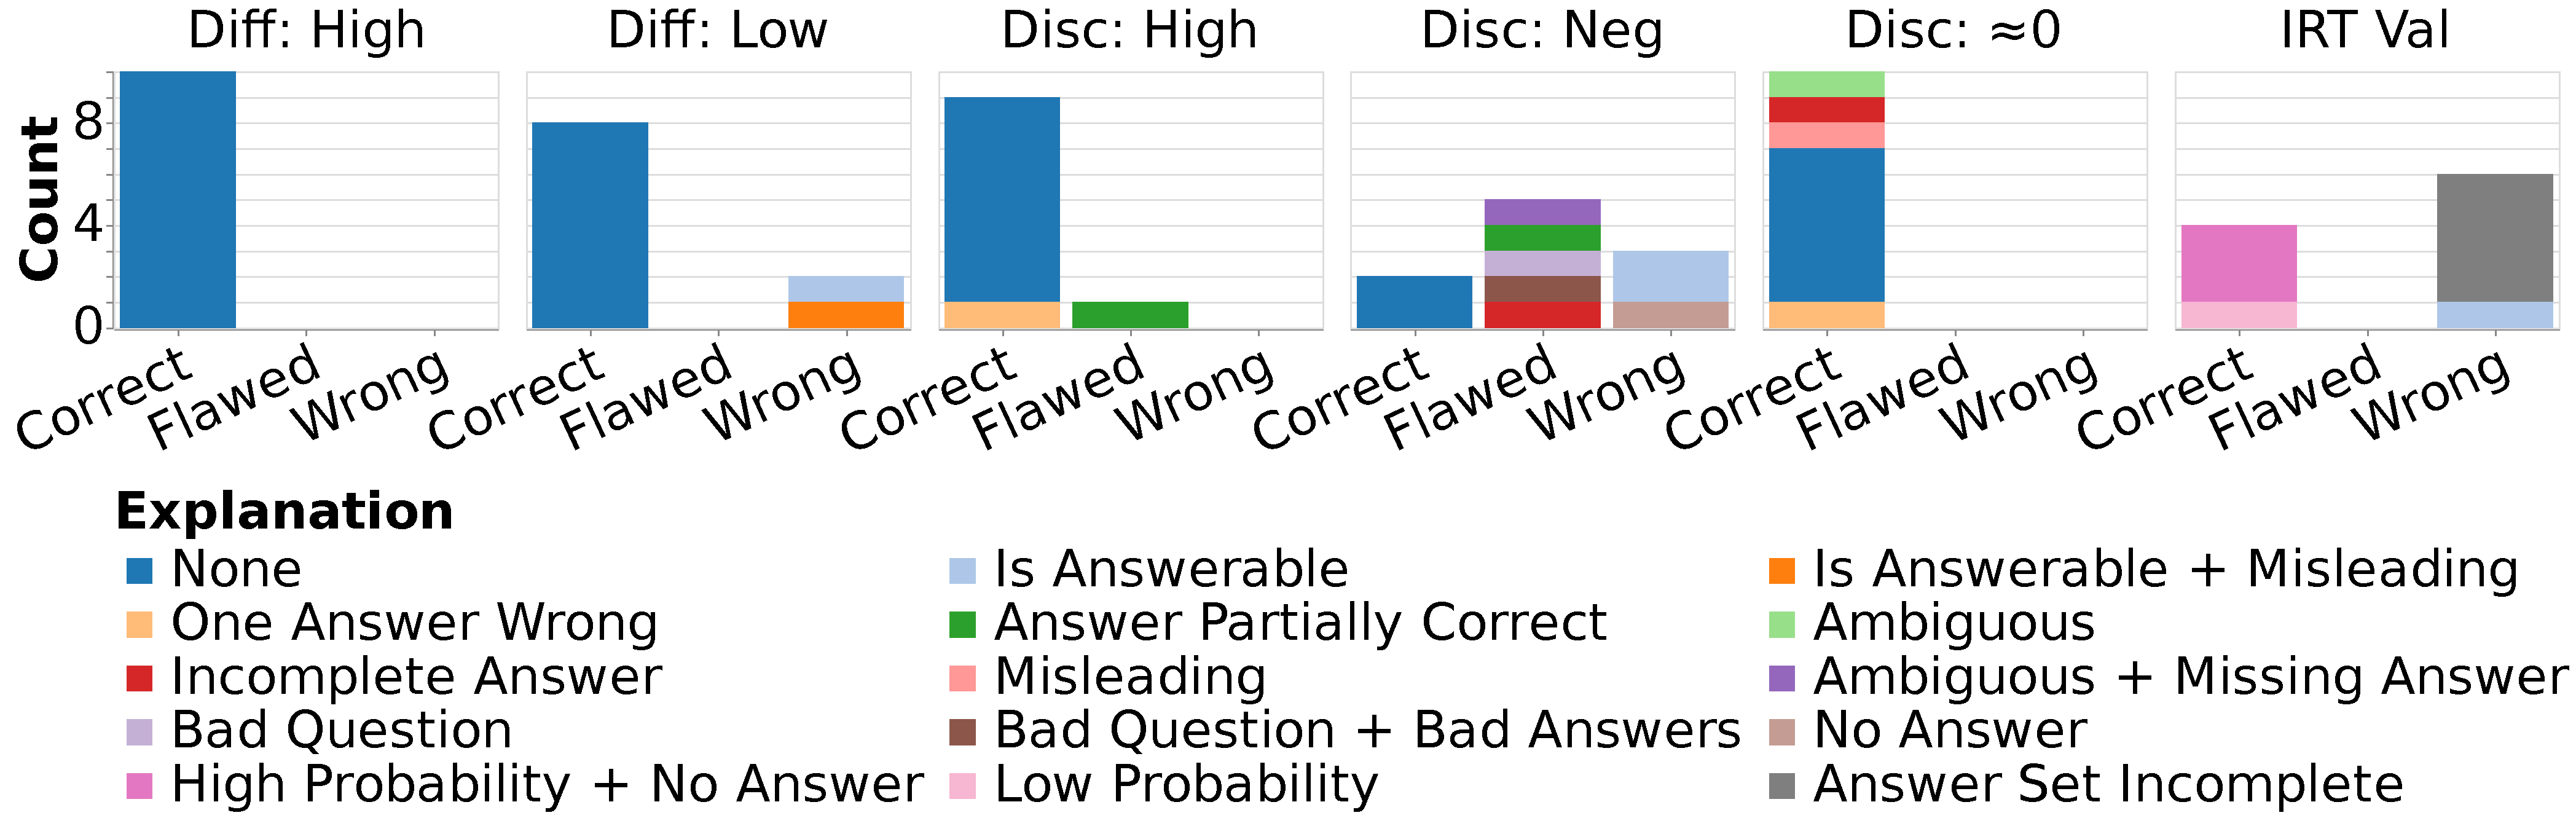
\includegraphics[width=\textwidth]{example_analysis.pdf}
    \caption{
        We annotate \squad{} \itms{} by \discability{}, \diff{}, and \irt{} prediction errors.
        For example, one question with negative \discability{} was classified as ``Wrong'' with the explanation that the annotated answer indicates it is \iemph{not} answerable, but the question actually \iemph{is} answerable.
        \Itms{} with negative \discability{} or where \irt{}'s prediction is wrong have a much higher rate of annotation error (``Flawed'' or ``Wrong'').
        Using similar methodology, errors in datasets could be more rapidly identified.
    }
    \label{fig:example-error}
\end{figure*}
